\documentclass[a4paper,12pt]{article}
\usepackage{styles}

\title{Analysis of FID shapes of Solids in glassy condition}
\author{Baranauskaite Valeriia, Mariia Ivanova, Leonid's Sister, Leonid Grunin}


\begin{document}


\section*{План статьи}
\subsection*{Введение}
\begin{enumerate}
  \item Какую информацию об образце мы можем получить, используя метод ЯМР в низких полях?
  \item О молекулярных движениях, как источнике информации, с точки зрения ЯМР-релаксометрии. О видах движения (работы Кая).
  \item О влиянии времени корреляции на T1, T2 твердых и жидких фаз образцов и форму спектральной линии.
  \item Корреляция структуры и свойств веществ с амплитудными и временными характеристиками спадов и параметров спектра.
  \item Микрообзор того, что кто смотрит по фиду.
  \item ГЭП – разброд и шатание в подходах к обработке фидов.
  \item Цель работы.
\end{enumerate}
\subsection*{Результаты и Дискуссия}
\begin{enumerate}
  \item Твердые тела. Подбор ЯМР-экспериментов с кратким описанием их особенностей.
  \item Обработка данных во временной области.
  \item Модели Абрагам, Гаусс, Вейбулл, Эксп. в зависимости от молекулярной динамики. Комбинации моделей в гетерофазных образцах. Модели не всегда идеально подходят – наши экспериментальные данные по разным видам твердых образцов.
  \item Обработка данных в частотной области.
  \item Формы спектральных линий. Второй момент. Взаимосвязь второго момента с временем поперечной релаксации.
  \item Новый метод: Second moment approximation.
  \item Идея.
  \item Примеры применения к спадам с осцилляцией и без.
  \item Сопоставление с результатами подходов Интегрирования и Усреднения.
  \item Возможные будущие задачи. Может, как-то корреляцию с DQ поизучать.
  \item Медленные движения молекул твердых тел эффективнее исследовать по спаду свободной индукции.
  \item Есть модификации как RK, Solid Echo (самые сильные дипольные взаимодействия), MSE (вроде, слабые).
  \item На каждом из упомянутых экспериментов по-разному отражается константа остаточных дипольных взаимодействий.
\end{enumerate}

\maketitle %to insert the title in the document
\section*{Abstract}

Why is it important\\
What has been done\\
What was found\\
What is the general result\\
How it can be used in the future\\

\newpage
\section{Introduction}

\newpage
\section{Experiment details}

\newpage
\section{Results and discussion}\label{sec:Results and discussion}
\subsection{FID processing in Time-Domain NMR}\label{sec:FID processing in Time-Domain NMR}

The recorded FID signal in NMR experiments typically consists of time, and real and imaginary components. 
Before analyzing the shape of FID, it undergoes preprocessing steps, including baseline subtraction, phase and frequency adjustments in the time domain.
The NMR signal for baseline is recorded in the empty ampule at exactly the same conditions as the sample. 
Phase adjustment addresses phase errors in the time domain data. 
These errors can arise from imperfections in the experimental setup or sample characteristics. 
The process involves finding the optimal phase angle that minimizes the difference between the real component of the FID signal and the overall amplitude of the signal within the initial part (typically before 30 microseconds). 
By adjusting the phase angle, we aim to align the real component of the signal with its amplitude, ensuring accurate representation of the signal's characteristics.

Frequency adjustment ensures that the frequency spectrum of the signal is correctly positioned and scaled.
This adjustment is crucial due to potential imperfections in the equipment or sample, which can cause the signal to deviate from its ideal state. 
The Fast Fourier Transform (FFT) procedure transforms the normalized time-domain signal into a frequency-domain in the form of a spectrum. 
The frequency axis is determined based on the time axis, following the Nyquist theorem. 
The spectrum is then shifted so that the maximum aligns with zero frequency, ensuring an even representation of positive and negative frequencies, i.e. symmetric spectrum. 
Finally, an inverse FFT (iFFT) is performed to obtain the FID signal with the corrected frequency.

\begin{figure}[H]
  \centering
  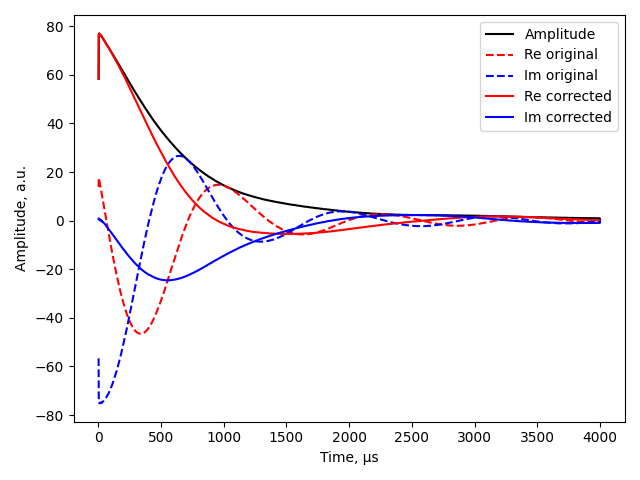
\includegraphics[width=10cm]{images/Original_Corrected_FID.png}
  \caption{The comparison between original (solid lines) and corrected (dashed lines) signals}
  \label{fig:Original_Corrected_FID}
\end{figure}

To mitigate the effects of magnet inhomogeneity at short time scales (before $30 \mu s$), where the fast relaxation occurs, it is recommended to subtract the long component. 
Glycerol, known for its long relaxation times, serves as a suitable reference. 
Alternatively, any substance with a transverse relaxation time exceeding 2 milliseconds can be used. 
The Glycerol's reference FID is normalized, adjusted for frequency and phase in the same manner as it was done with Sample. 
Subsequently, the real component of the Sample is divided by the amplitude of the Glycerol FID.

To eliminate the long component, an exponential fitting of the real part of the FID corresponding to the slow decay within the time range before $200 \mu s$ should be conducted and the fitted curve should be subtracted from the original data.

\begin{figure}[H]
  \centering
  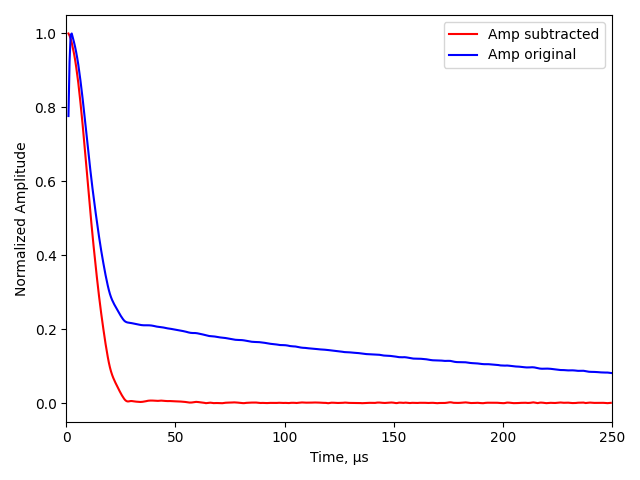
\includegraphics[width=10cm]{images/Subtracted_FID.png}
  \caption{The comparison of the original FID (red) and subtracted FID (blue)}
  \label{fig:Subtracted_FID}
\end{figure}

The concluding steps in the time-domain involve apodizing the real and imaginary components of the FID, followed by zero-filling to ensure that the final FID comprises a power of 2 number of data points ($2^n$). 
This step is crucial as FFT computation is more efficient with data containing this specific number of points. 
Subsequently, the FFT procedure is applied, yielding the resulting spectrum in the frequency-domain.

\begin{equation}
  \label{eq:apodization}
  f(apodization) = \exp\left(-\left[\frac{Time}{\sigma}\right]^4\right)
\end{equation}


\subsection{FID processing in Frequency-Domain NMR}\label{sec:FID processing in Frequency-Domain NMR}

The spectra derived from the FFT procedure can be manually phased using linear or polynomial functions.
Subsequently, the resulting real and imaginary components of the spectra can be recalculated accordingly. 

\begin{equation}
  \label{eq:amplitude calculation}
  \begin{split}
Re = Re \cdot \cos(\phi) - Im \cdot \sin(\phi)\\
Im = Re \cdot \sin(\phi) + Im \cdot \cos(\phi)\\
Amplitude = \sqrt{Re^2 + Im^2}
  \end{split}
\end{equation}

Additionally, apodization of the spectrum, akin to the time-domain signal, should be performed to ensure zero amplitude at high frequencies, utilizing similar equations as in \cref{eq:apodization}. 
Once apodized, the acquired spectrum is prepared for further analysis, such as the calculation of the second moment.


\newpage
\section{Conclusions}

\newpage
\section{References}
\printbibliography

\end{document}
